\subsection{Project Description}

\par This project will deliver a web application that will be used to interactively visualize biodiversity data.
This application will be used by researchers and Department of Defense land managers to compare and analyze biodiversity data in areas of interest.

\subsection{Service Need}

\par Professionals working out in the field on government-owned property are tasked with preserving the ecosystems within them.
To serve this purpose, they’ve requested a tool with which they can quickly assess biodiversity levels of different key areas.

\subsection{Client Requirements}

\par Our client will provide us with the data to visualize and a web server on which to host the application.
\begin{list}{-}{}
\item The dataset will provide each individual observation of an insect, including the location, time, and taxa of the species observed.
\begin{list}{-}{}
\item The location will be one of about 700 sites in the Southwestern United States, and will include latitude and longitude.
Sites are hierarchically organized in that each site belongs to a basin.
\item The time will be between 2009 and 2013.
Samples were collected at individual sites anywhere from only once to twice a year.
\item The taxa will be the fully qualified taxonomy of the insect species observed.
These will be hierarchically organized, as every species belongs to a genus, which belongs to a family, and order, and so on.
\end{list}
\end{list}

\subsection{Functional Requirements}

\par We will create a web interface for interacting with and visualizing the dataset provided to us.
This interface will provide three views:

\begin{list}{-}{} % main list

\item Map View

\begin{list}{-}{}
\item This view will display a map, annotated with markers at the locations of all the sites where data have been collected.
\item Users will be able to pan and zoom in this view.
\item They will also be able to select a site in this view by clicking on it.
\item As a stretch goal, we will display markers with size or color according to biodiversity metrics of that site.
\end{list}

\item Statistics View

\begin{list}{-}{}
\item This view will display useful summary statistics, graphs, and charts about the selected information.
These will include:
\begin{list}{-}{}
\item A graph of biodiversity over time.
\item The Shannon diversity score.
\item A chart of insect population by taxa or species.
\end{list}
\end{list}

\item Filter view
\begin{list}{-}{}
\item This view will allow the user to filter what information is displayed in the Map and Statistics Views.
It will contain:
\begin{list}{-}{}
\item Date filter
\begin{list}{-}{}
\item This will allow the user to select data from a range of dates.
\end{list}
\item Taxa filter
\begin{list}{-}{}
\item This will allow the user to select multiple taxa (e.g. species, order).
\item The species will be organized hierarchically within the pane.
\end{list}
\item Site filter
\begin{list}{-}{}
\item This will allow users to select multiple sites.
\item The sites will be organized hierarchically (into their containing basins) within the pane.
\end{list}
\end{list}
\end{list}

\item STRETCH GOAL Advanced statistical analysis
\begin{list}{-}{}
\item As a stretch goal, this feature will go beyond the data manipulation implemented in the different graphing features of the main app.
We will work with David Lytle and his team to generate advanced statistical models on the data they’ve gathered.
Since this is a stretch goal, it is currently undefined and will only be reached once we complete the 1.0 version of our website.
\end{list}
\end{list}

\subsection{Technical Requirements}

\begin{list}{-}{}
\item Set up mapping tool
\begin{list}{-}{}
\item Set up a mapping tool (e.g. ArcGIS) to create the map view.
\end{list}
\item Test cross-browser support
\begin{list}{-}{}
\item We will test our application to support common browsers such as Chrome, Firefox, Internet Explorer, and Edge.
\end{list}
\item Set up web server
\begin{list}{-}{}
\item We will set up a web server to host our application. We will either acquire a server or use a web hosting service.
\end{list}
\item Set up website
\begin{list}{-}{}
\item We will create a base website to house our application.
We will build this with a web framework to do the heavy lifting for basic needs such as user control, security, database access, and templating.
\end{list}
\item Set up database
\begin{list}{-}{}
\item We will get this data in its raw form from our client.
We will then convert their data into a form that can be stored in a relational database.
\end{list}
\item Create In-depth documentation
\begin{list}{-}{}
\item We will provide sufficient technical documentation of our application for another developer to make extensions and additions to it.
\end{list}
\end{list}

\subsection{Communication Plan}
\par We will use the following for our internal communication:
\begin{list}{-}{}
\item Slack
\begin{list}{-}{}
\item We will use this chat client for coordinating meeting times.
\end{list}
\item GitHub
\begin{list}{-}{}
\item We will keep version control of our code on GitHub.
\end{list}
\item Regular meetings several times a week
\begin{list}{-}{}
\item In order to make regular process towards goals that have been assigned and set by ourselves, we will meet regularly and consistently re-evaluate our progress.
\end{list}
\end{list}

\par We will use the following for our external communication:
\begin{list}{-}{}
\item Email will be our primary means of contact with our client.
\item We will meet twice a month with our TA.
\item We will meet twice a month with our client.
\end{list}

\subsection{Documentation}
\par Technical Documentation will be provided by the following:
\begin{list}{-}{}
\item Microsoft Sharepoint
\begin{list}{-}{}
\item As per our class requirements, we’ve created a sharepoint site that will be the primary form of providing updates on progress and holding all revisions of our code base and documentation.
This is shared amongst the client, the developer team, and the professor/TAs.
\end{list}
\item Github
\begin{list}{-}{}
\item While the sharepoint site will be where all code versions will be hosted officially, Github will be the tool the development team will use for version control internally.
Documentation will be held here as well, but replicated in the sharepoint site.
\end{list}
\end{list}

\subsection{Timeline}
Timeline showed in Fig \ref{fig:original_gantt}.
\begin{figure}[h]
\centering
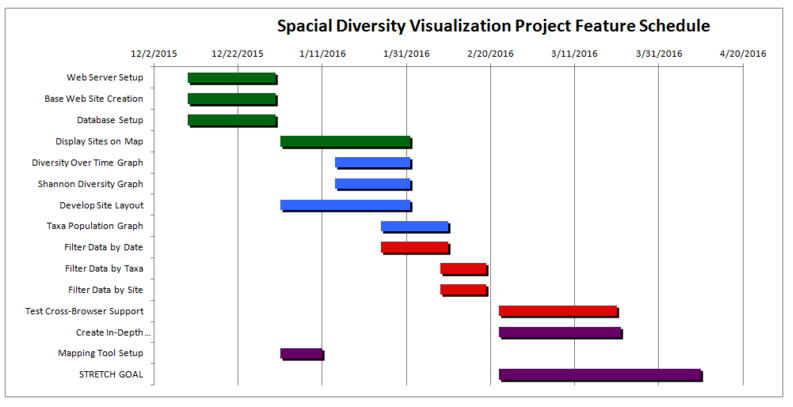
\includegraphics[width=0.9\textwidth]{OriginalGantt.png}
\captionsetup{justification=centering}
\caption{
  This is our original speculated gantt chart.
  It displays the time estimates that we had originally assumed various required tasks would take.
  As you can see it had a fairly smooth flow to it, which we learned soon in was very different in practice.
}
\label{fig:original_gantt}
\end{figure}

\subsection{Signature}
This looks good to me as a starting document. It doesn't have much about the Obj 2 statistical parts, but we can add those later. Consider this email my signature on the document.
Dave+
*************************************
David A. Lytle
Oregon State University
(541) 737-1068
